\section{String Diagram Rewrite Theory}%
\label{sec:combinatorial-semantics}

We recall the fundamental definitions and results of string diagram rewrite theory for symmetric monoidal categories, recapitulating the correspondence between string diagram rewriting and an appropriate notion of double pushout (DPO) rewriting of certain hypergraphs, as established in~\citet{bonchi_string_2022-1, bonchi_string_2022-2}.

First,  we fix some notation.  Let $(-)^*$ be the free monoid monad over $\catname{Set}$.
We extend this to the case of relations $R \subseteq V \times V$,  denoting by $R^{*} \subseteq V^* \times V^*$ the element-wise extension of $R$ to a relation on ordered sequences.
We will sometimes use functional notation for relations, so that given $R \subseteq V \times W$ and $v \in V$, we write $R(v) \in W$.
We elide associativity and unit isomorphisms associated with coproducts $\sqcup$,  and denote by $\iota_j\colon X_{j} \rightarrow X_{1} \sqcup \dots X_{j} \sqcup \dots X_{n}$ the $j^{\text{th}}$ injection,  and $[f,g]\colon A_1 \sqcup A_2 \to B$ the co-pairing of two morphisms $f\colon A_1 \to B$ and $g\colon A_2 \to B$.
We denote by $A \sqcup_{f,g} B$ the pushout of the span $A \xleftarrow{f} C \xrightarrow{g} B$.
We will also refer to $A,B$ as \emph{feet} of the cospan, and to $C$ as \emph{carrier}.
% Given an ordered sequence of labels from some alphabet $\Sigma$, $[l_1, \ldots, l_n]$ we will denote with $w([l_1, \ldots, l_n])$ the word concatenated from these labels using $\otimes$, e.g.\ $w([A,B]) = A \otimes B$.

\subsection{Hypergraphs}

Hypergraphs generalise directed graphs by allowing edges to have multiple (ordered) sources and targets.
\citet{bonchi_string_2022-2} show that a certain class of hypergraphs \emph{with interfaces} and their DPO rewriting are sound and complete for categorical presentations of arbitrary symmetric monoidal theories.
Moreover, they develop the use of hypergraphs as combinatorial representations of string diagrams for symmetric monoidal categories, whereby morphisms (nodes) are represented as hyperedges, and objects (wires) as vertices.
We briefly present this correspondence, but the interested reader should consult the work of~\citet{bonchi_string_2022-1,bonchi_string_2022-2}.

\begin{definition}[Category of hypergraphs]\label{def:hypergraph}
	Over a monoidal signature $\Sigma = (\Sigma_{O}, \Sigma_{M})$, a hypergraph $\mathcal{G}$ is a tuple $(V,E,s,t,l)$, where $V$ is a finite set of vertices, $E$ is a finite set of hyperedges, $s\colon E \to V^{*}$ is a source function, $t\colon E \to V^{*}$ is a target function,  and $l = (l_{V}\colon V \to \Sigma_{O},l_{E}\colon E \to \Sigma_{M})$ is a pair of labelling functions that assigns each hyperedge and vertex an operator and a type from monoidal signature $\Sigma$ respectively.

	The labelling function must respect the typing of the operator:
	\[
		\forall e \in E. \, l(e) = c : A \to B \implies l_{V}^{*}(s(e)) = A \text{ and } l_{V}^{*}(t(e)) = B.
	\]
	We call a hypergraph discrete if its set of hyperedges is empty.

	A \emph{hypergraph homomorphism} $\phi\colon \mathcal{F} \to \mathcal{G}$ is given by a pair of functions $\phi_V\colon V_{\mathcal{F}} \to V_{\mathcal{G}}, \phi_E\colon E_{\mathcal{F}} \to E_{\mathcal{G}}$ such that the following hold:
	\begin{align*}
		\phi_V^*(s_{\mathcal{F}}(e)) & = s_{\mathcal{G}}(\phi_E(e)),   & \phi_V^*(t_{\mathcal{F}}(e)) & = t_{\mathcal{G}}(\phi_E(e)),   \\
		l_{V,\mathcal{F}}(v)         & = l_{V,\mathcal{G}}(\phi_V(v)), & l_{E,\mathcal{F}}(e)         & = l_{E,\mathcal{G}}(\phi_E(e)).
	\end{align*}

	We denote by $\catname{Hyp(\Sigma)}$ the category of hypergraphs over $\Sigma$ and hypergraph homomorphisms.
\end{definition}
$\catname{Hyp(\Sigma)}$ is equivalently characterised as the category of (finite) presheaves over the category $\mathbf{I}$ generated by objects pairs $(k, l) \in \mathbb{N} \times \mathbb{N}$ and an additional object $\star$, with $k + l$ morphisms: $\{ i\colon \star \to (k, l) \mid 0 \leq i < k + l \}$.
As such, it has all finite colimits; the initial object is given by the empty hypergraph, and coproducts are given by the disjoint union of hypergraphs.

However, there is also a need to specify which vertices are to be considered as \emph{input} and \emph{outputs} to the diagram as a whole, corresponding to the dangling wires exiting at the top and bottom of a string diagram.
This gives rise to the definition of a hypergraph with interfaces via a construction on cospans.

% \begin{definition}[Symmetric monoidal category of cospans]
% Let $\mathbb{C}$ be a category with all finite colimits.  
% A cospan from $X$ to $Y$ is a pair of arrows $X \xrightarrow{} A \xleftarrow{} Y$  in $\mathbb{C}$.  This \emph{category of cospans of $\mathbb{C}$},  denoted $\catname{Csp(\mathbb{C})}$,  has as objects those of $\mathbb{C}$ and as arrows isomorphism classes of cospans.

% Composition of cospans $X \xrightarrow{f} A \xleftarrow{g} Y$ and $Y \xrightarrow{h} B \xleftarrow{i} Z$ is given by pushout: $X \xrightarrow{f} A \sqcup_{g,h} B \xleftarrow{i} Z$,  with identity given by the cospan of identities.  Its monoidal product is given by the coproduct of $\mathbb{C}$ as follows: 
% \begin{multline*}
%     (A \xrightarrow{f} \mathcal{G} \xleftarrow{g} B) \otimes (A^\prime \xrightarrow{f^\prime} \mathcal{G^\prime} \xleftarrow{g^\prime} B^\prime) \coloneq\\ A \sqcup A^\prime \xrightarrow{f \sqcup f^\prime} \mathcal{G} \sqcup \mathcal{G^\prime} \xleftarrow{g \sqcup g^\prime} B \sqcup B^\prime  , 
% \end{multline*}
% and its unit by the initial object of $\mathbb{C}$.
% Symmetry is inherited from $\mathbb{C}$ as the coproduct~\cite{MonoidalCoproduct}.
% \end{definition}

% Then, morphisms of $\catname{S}(\Sigma)$ can be interpreted as particular cospans of discrete hypergraphs,  which we call hypergraphs with interfaces~\cite{bonchi_string_2022-2}.
\begin{definition}[Hypergraphs with interfaces]%
	\label{def:cspd}
	A hypergraph with interfaces is a cospan $n \xrightarrow{f} \mathcal{G} \xleftarrow{g} m$ in $\catname{Hyp}(\Sigma)$ where $n$, $m$ are discrete hypergraphs denoting input and output interfaces.
	Write $\catname{HypI}(\Sigma)$ for the full subcategory of the quotient category of cospans\footnote{This is the 1-categorical version of the bicategory of cospans: for a bicategory, its quotient category is given by the same objects but by taking \emph{isomorphism classes} of morphisms instead.} of $\catname{Hyp}(\Sigma)$ whose objects are discrete hypergraphs and morphisms are isomorphism classes of cospans of hypergraphs\footnote{By abuse of notation, we ignore the distinction between a cospan and its isomorphism class --- this is validated by replacing \enquote{pushout} (which is only determined up to unique isomorphism) by \enquote{chosen pushouts}, which any concrete setting (e.g.\ an implementation of DPO rewriting) would satisfy.}.
\end{definition}
$\HypI{\Sigma}$ is a symmetric monoidal category:
\begin{enumerate}
	\item the tensor product given by coproduct in $\catname{Hyp}(\Sigma)$:
	      \begin{align*}
		      n \xrightarrow{f}               & \mathcal{F} \xleftarrow{g} m                                                                                                                                       \\
		                                      & \otimes \qquad \quad \Coloneqq n \sqcup n^\prime \xrightarrow{f \sqcup f^\prime} \mathcal{F} \sqcup \mathcal{G} \xleftarrow{g \sqcup g^\prime} m \sqcup m^\prime ; \\
		      n^\prime \xrightarrow{f^\prime} & \mathcal{G} \xleftarrow{g^\prime} m^\prime
	      \end{align*}
	\item the monoidal unit is given by the initial object of $\catname{Hyp}(\Sigma)$;
	\item symmetry is inherited from coproduct in $\catname{Hyp}(\Sigma)$~\cite{MonoidalCoproduct}.
\end{enumerate}

Composition of two cospans $n \xrightarrow{f} \mathcal{F} \xleftarrow{g} m;m \xrightarrow{f^\prime} \mathcal{G} \xleftarrow{g^\prime} k$ is given by the pushout
$
	n \xrightarrow{f} \mathcal{F} \sqcup_{g,f^\prime} \mathcal{G} \xleftarrow{g^\prime} k
$,
computed by identifying vertices in $\mathcal{F} \sqcup \mathcal{G}$ that share pre-image in $m$.

As it stands, every string diagram in a symmetric monoidal category can be represented by a hypergraph with interfaces, but the converse is not true.
In order to rectify this, we impose additional constraints on the hypergraphs under consideration.
\begin{definition}[Degree,  path,  acyclic]
	The in-degree of a vertex $v$ in a hypergraph $\mathcal{G}$ is the number of hyperedges $e \in {E_\mathcal{G}}$ such that $v \in t(e)$.
	Similarly, the out-degree of $v$ is the number of hyperedges $e \in E_\mathcal{G}$ such that $v \in s(e)$.
	A path from $e_0$ to $e_{n-1}$ of length $n$ in a hypergraph $\mathcal{G}$ is an ordered sequence of hyperedges $[e_0, e_1, \ldots, e_{n-1}] \in E_\mathcal{G}^*$ such that for all $i < n - 1$ some vertex $v \in t(e_i)$ is also in $s(e_{i+1})$.
	A hypergraph is directed acyclic if it contains no paths of length $n > 0$ that start and end in the same hyperedge.
\end{definition}

\begin{definition}[Category of MDA Hypergraphs with Interfaces~\cite{bonchi_string_2022-2}]%
	\label{def:monogamy_hyp}
	We call a cospan $n \xrightarrow{f} \mathcal{G} \xleftarrow{g} m$ in $\HypI{\Sigma}$ monogamous if:
	\begin{enumerate}
		\item $f$ and $g$ are monomorphisms;
		\item the in-degree and out-degree of every vertex is at most~$1$;
		\item vertices with in-degree $0$ are precisely the image of $f$;
		\item vertices with out-degree $0$ are precisely the image of $g$.
	\end{enumerate}
	We denote by $\MdaCospans$ the subcategory of $\HypI{\Sigma}$ of monogamous directed acyclic (MDA) cospans.
\end{definition}

\autoref{fig:hypergraph-with-interfaces} gives an example of an MDA cospan, which is such because it \enquote{looks like} the string diagram \comonoid.
Analogously, we can see that~\autoref{fig:hypergraph} (equipped with the interfaces choosing $\{ v_1 \}$ and $\{ v_4, v_5, v_6, v_7 \}$) fails to form an MDA cospan --- it is not monogamous for many reasons: $v_1$ has out-degree 0, $v_1, v_5, v_7$ have in-degree 2, and $v_3$ has in-degree 0; additionally, it fails be be directed acyclic due to the path along $e_4$ from $v_7$ to itself\footnote{Recall that loops are not part of the syntax of string diagrams for symmetric monoidal categories in the absence of a trace --- a relaxation of monogamy to allow for this is explored by~\citet{ghica_rewriting_2023}.}.

\begin{figure}
	\begin{subfigure}[c]{0.3\linewidth}
		\centering
		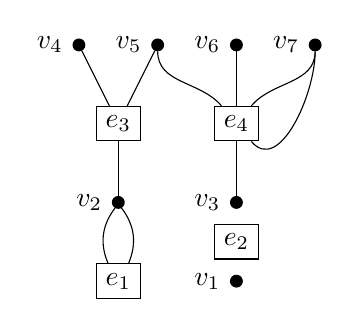
\begin{tikzpicture}[
				vertex/.style={draw, circle, fill, inner sep=1.5pt},
				hyperedge/.style={draw, rectangle}
			]
			\node[vertex, label=left:{$v_4$}] (v1) at (0,0) {};
			\node[vertex, label=left:{$v_5$}] (v2) at (1,0) {};
			\node[vertex, label=left:{$v_6$}] (v3) at (2,0) {};
			\node[vertex, label=left:{$v_7$}] (v4) at (3,0) {};
			\node[vertex, label=left:{$v_2$}] (v5) at (0.5,-2) {};
			\node[vertex, label=left:{$v_3$}] (v6) at (2,-2) {};
			\node[vertex, label=left:{$v_1$}] (v7) at (2,-3) {};

			\node[hyperedge] (e1) at (0.5,-1) {$e_3$};
			\node[hyperedge] (e2) at (2,-1) {$e_4$};
			\node[hyperedge] (e3) at (0.5,-3) {$e_1$};
			\node[hyperedge] (e4) at (2,-2.5) {$e_2$};

			\draw (v1) -- (e1);
			\draw (v2) -- (e1);
			\draw (v5) -- (e1);
			\draw (v5) edge[bend right] (e3);
			\draw (v5) edge[bend left] (e3);
			\draw (v2) edge[in=130,out=-90] (e2);
			\draw (v3) -- (e2);
			\draw (v4) edge[in=50,out=-90] (e2);
			\draw (v4) edge[in=-50,out=-90] (e2);
			\draw (v6) -- (e2);
		\end{tikzpicture}
		\caption{Hypergraph with 7 vertices and 4 hyperedges, all directed bottom-to-top; source/target vertices are ordered left-to-right.}%
		\label{fig:hypergraph}
	\end{subfigure}
	\begin{subfigure}[c]{0.3\linewidth}
		\centering
		\begin{tikzpicture}[
				vertex/.style={draw, circle, fill, inner sep=1.5pt},
				hyperedge/.style={draw, rectangle}
			]
			\node[vertex, label=left:{$v_3$}] (v1) at (0,0) {};
			\node[vertex, label=left:{$v_3$}] (v1') at (0,1.5) {};
			\node[vertex, label=left:{$v_2$}] (v2) at (1,0) {};
			\node[vertex, label=left:{$v_2$}] (v2') at (1,1.5) {};
			\node[vertex, label=left:{$v_1$}] (v3) at (0.5,-2) {};
			\node[vertex, label=left:{$v_1$}] (v3') at (0.5,-3.5) {};

			\node[hyperedge] (e1) at (0.5,-1) {$e_1$};

			\draw (v1) -- (e1);
			\draw (v2) -- (e1);
			\draw (v3) -- (e1);

			\node[draw, rounded corners, fit={(v1'.west) (v2'.west)}, inner sep=12pt] (S) {};
			\node[draw, rounded corners, fit={(v3'.west)}, inner sep=12pt] (T) {};
			\node[draw, rounded corners, fit={(v1.west) (v2.west) (v3.west)}, inner sep=12pt] (H) {};
			\draw[commutative diagrams/hookrightarrow,shorten >=2pt,shorten <=2pt] (S) -- node[left] {$g$} (H);
			\draw[commutative diagrams/hookrightarrow,shorten >=2pt,shorten <=2pt] (T) -- node[left] {$f$} (H);
		\end{tikzpicture}
		\caption{Hypergraph with interfaces}%
		\label{fig:hypergraph-with-interfaces}
	\end{subfigure}
	\caption{Example hypergraphs}%
	\label{fig:hypergraph-examples}
\end{figure}

Note that $\MdaCospans$ remains a symmetric monoidal category with the same structure as before.
We now recall the following theorem~\cite{bonchi_string_2022-2}, which says there is a symmetric monoidal equivalence which witnesses that MDA hypergraphs with interfaces are precisely string diagrams.
\begin{theorem}[Corollary 26 of~\cite{bonchi_string_2022-2}]\label{thm:prop-equiv}
	$\catname{S}(\Sigma) \cong \MdaCospans$
\end{theorem}

The practical meaning of this is that two $\Sigma$-terms $f$ and $g$ are equal modulo symmetric monoidal category equations if and only if they are represented as the same hypergraph with interfaces.
The theorem defines a full and faithful functor that is induced by the interpretation function of morphism terms that renders the latter as cospans of hypergraphs and is given in~\autoref{sec:appendix:interpretation}.
Term rewriting and hence equality modulo $\mathcal{E}$ is then implemented as DPO rewriting over such hypergraphs with interfaces, which we recall next.

\subsection{DPOI-Rewriting for Hypergraphs with Interfaces}
DPO rewriting is a standard technique for formalising graph transformations categorically.
% In this section we recall standard results of double-pushout (DPO) rewriting of hypergraphs,  as well as the specific notion of DPO rewriting which is sound and complete for arbitrary SMTs,  which is called \emph{convex} rewriting.
The intuitive notion of (hyper-)graph rewriting is  as expected: given a rewrite rule $\mathcal L \rightsquigarrow \mathcal R$ and a graph $\mathcal{G}$,  we expect to find an occurrence of $\mathcal L$ within $\mathcal{G}$,  remove it,  and then plug $\mathcal R$ into the hole to determine the rewritten graph $\mathcal{H}$.
In DPO rewriting, such a rewrite rule is formalised as a span $\mathcal L \xleftarrow{} \mathcal K \xrightarrow{} \mathcal R$ in some appropriate category of graphs, where $\mathcal{K}$ is some invariant graph fragment that should be maintained during rewriting.
A typical DPO square is depicted in~\autoref{fig:dpo_dpoi}~(left).

The morphism $\mathcal{L} \to \mathcal{G}$ is called a \emph{match}, defined whenever there is a corresponding \emph{pushout complement} --- the pair of morphisms $\mathcal{K} \to \mathcal{L}^{\bot} \to \mathcal{G}$ completing the top half of the pushout square with $\mathcal K \xrightarrow{} \mathcal L \xrightarrow{} \mathcal G$.
When the morphisms involved in the rewrite rule are monomorphisms, as is usually required, constructing $\mathcal{L}^{\bot}$ can be intuitively understood as finding an occurrence of $\mathcal{L}$ in $\mathcal{G}$ and removing from this occurrence everything that has no preimage in $\mathcal{K}$.
The final graph $\mathcal H$ is then obtained by inserting into the hole everything from $\mathcal{R}$ that has no preimage in $\mathcal{K}$ --- hence the two pushouts: one for deletion and one for insertion.
In this case, we say that $\mathcal{G}$ is rewritten into $\mathcal{H}$ via the rewrite rule $\mathcal{L} \xleftarrow{} \mathcal{K} \xrightarrow{} \mathcal{R}$.

To express the rewriting of (hyper-)graphs with interfaces,  i.e.\ the ones that represent morphisms in $\HypI{\Sigma}$, the DPO formalism has been extended to double-pushout rewriting with \emph{interfaces} (DPOI) as shown in~\autoref{fig:dpo_dpoi}~(right).
In the case of $ \catname{Hyp(\Sigma)}$,  we wish for a rewrite rules to be pairs of discrete cospans of hypergraphs with matching interfaces: $n \xrightarrow{} \mathcal{L} \xleftarrow{} m$, $n \xrightarrow{} \mathcal{R} \xleftarrow{} m$.
By noting that a cospan $0 \xrightarrow{} \mathcal{L} \xleftarrow{[f,g]} n \sqcup m$ encodes the same data as a cospan $n \xrightarrow{f} \mathcal L \xleftarrow{g} m$ \cite[Remark 3.14]{bonchi_string_2022-1} we can formulate a rewrite rule as a single span $\mathcal{L} \xleftarrow{} n \sqcup m \xrightarrow{} \mathcal{R}$,  and we can do similarly for the discrete cospans giving the interface to $\mathcal{G}$ and $\mathcal{H}$.
We now make this identification throughout without further mention.
Thus, we reach the following variant of DPO rewriting.
\begin{definition}[DPOI rewriting]%
	\label{def:dpoi}
	Given a span of morphisms $\mathcal{G} \xleftarrow{} n \sqcup m \xrightarrow{} \mathcal{H}$ in $\catname{Hyp}(\Sigma)$,  we say $\mathcal{G}$ rewrites to $\mathcal{H}$ with interface $n \sqcup m$ via rewrite rule $\mathcal{L} \xleftarrow{} i \sqcup j \xrightarrow{} \mathcal{R}$ if there exists an object $\mathcal{C}$ and morphisms which complete the rightmost commutative diagram in~\autoref{fig:dpo_dpoi} such that the two marked squares are pushouts.

	\begin{figure}[t!]
		\begin{subfigure}[T]{0.35\linewidth}
			\[
				% \tikzfig{../figures/combinatorial_semantics/DPO_square}
				\begin{tikzcd}
					{\mathcal{L}} & {\mathcal{K}} & {\mathcal{R}} \\
					{\mathcal{G}} & {\mathcal{L}^{\bot}} & {\mathcal{H}}
					\arrow["f"', from=1-1, to=2-1]
					\arrow[from=1-2, to=1-1]
					\arrow[from=1-2, to=1-3]
					\arrow[from=1-2, to=2-2]
					\arrow[from=1-3, to=2-3]
					\arrow["\lrcorner"{anchor=center, pos=0.125, rotate=90}, draw=none, from=2-1, to=1-2]
					\arrow[from=2-2, to=2-1]
					\arrow[from=2-2, to=2-3]
					\arrow["\lrcorner"{anchor=center, pos=0.125, rotate=180}, draw=none, from=2-3, to=1-2]
				\end{tikzcd}
			\]
			% \subcaption{DPO square}
			% \label{fig:dpo}
		\end{subfigure}
		\hfill
		\begin{subfigure}[T]{0.4\linewidth}
			\[
				% \scalebox{0.8}{
				% \tikzfig{../figures/combinatorial_semantics/DPOI_square_Hyp}
				% }
				\begin{tikzcd}
					{\mathcal{L}} & {i \sqcup j} & {\mathcal{R}} \\
					{\mathcal{G}} & {\mathcal{L}^{\bot}} & {\mathcal{H}} \\
					& {n \sqcup m}
					\arrow["f"', from=1-1, to=2-1]
					\arrow[from=1-2, to=1-1]
					\arrow[from=1-2, to=1-3]
					\arrow[from=1-2, to=2-2]
					\arrow[from=1-3, to=2-3]
					\arrow["\lrcorner"{anchor=center, pos=0.125, rotate=90}, draw=none, from=2-1, to=1-2]
					\arrow[from=2-2, to=2-1]
					\arrow[from=2-2, to=2-3]
					\arrow["\lrcorner"{anchor=center, pos=0.125, rotate=180}, draw=none, from=2-3, to=1-2]
					\arrow[from=3-2, to=2-1]
					\arrow[from=3-2, to=2-2]
					\arrow[from=3-2, to=2-3]
				\end{tikzcd}
			\]
			% \subcaption{DPOI square}
			% \label{fig:dpoi}
		\end{subfigure}
		\caption{DPO and DPOI squares}
		\label{fig:dpo_dpoi}
	\end{figure}

\end{definition}
To make DPOI rewriting sound and complete with respect to rewriting of $\Sigma$-terms modulo the laws of symmetric monoidal categories and equations $\mathcal{E}$, the notion of both pushout complement and match must be restricted: otherwise, there might be DPO rewrites that are not derivable.
This gives rise to the following notion of a \emph{boundary complement} and \emph{convex} DPOI rewriting.

\begin{definition}[Boundary complement]%
	\label{def:boundary_original}
	For MDA cospans $i \xrightarrow{a_1} \mathcal{L} \xleftarrow{a_2} j$ and $n \xrightarrow{b_1} \mathcal{G} \xleftarrow{b_2} m$ and monomorphism $f\colon \mathcal L \to \mathcal G$, a pushout complement $i \sqcup j \to \mathcal{L}^\bot \to \mathcal{G}$ as depicted in the square below
	\[
		\adjustbox{scale=0.8}{
			\tikzfig{./figures/DPOI_boundary_complement}
		}\]
	is called a boundary complement if $[c_1, c_2]$ is a monomorphism and there exist $d_1\colon n \to \mathcal{L}^{\bot}$ and $d_2\colon m \to \mathcal{L}^{\bot}$ making the above triangle commute and such that
	$
		n \sqcup j \xrightarrow{[d_1,c_2]} \mathcal{L}^{\bot} \xleftarrow{[d_2,c_1]} m \sqcup i
	$
	is an MDA cospan.
\end{definition}

Intuitively, requiring boundary complements ensures that inputs are glued exclusively to outputs and vice-versa in the two pushout squares.
% Yet, this restriction is not enough to make DPOI rewriting complete for $\catname{S}(\Sigma,\mathcal{E})$: there might be cospans with carriers $\mathcal{G}$ and $\mathcal{H}$ such that one can be rewritten into another but their corresponding morphisms are not equal modulo $\mathcal{E}$~\cite{bonchi_string_2022-2}.
% To make the DPOI rewriting complete, we need to add a restriction on the image of the match.

\begin{definition}[Convex match]
	A subgraph $\mathcal{H}$ of a hypergraph $\mathcal{G}$ is a convex subgraph if for all $v_i, v_j \in V_{\mathcal{H}}$ every path from $v_i$ to $v_j$ is also in $\mathcal{H}$.
	A match $f\colon \mathcal{L} \to \mathcal{G}$ is a convex match if it is a monomorphism and its image is a convex subgraph of $\mathcal{G}$.
\end{definition}

\begin{definition}[Convex DPOI rewriting]%
	\label{def:convex_dpo}
	Let $\mathfrak{R}$ be a set of DPOI rewrite rules.
	Then, given $\mathcal{G} \xleftarrow{} n \sqcup m$ and $\mathcal{H} \xleftarrow{} n \sqcup m$ in $\catname{Hyp(\Sigma)}$, $\mathcal{G}$ rewrites convexly into $\mathcal{H}$ with interface $n \sqcup m$, and we write $(\mathcal G \xleftarrow{} n \sqcup m ) \Rrightarrow_{\mathfrak{R}}  (\mathcal H \xleftarrow{} n \sqcup m )$, if
	\begin{enumerate}
		\item there exists a rule $\mathcal{L} \xleftarrow{} i \sqcup j \xrightarrow{} \mathcal{R}$ in $\mathfrak{R}$ and object $\mathcal{L}^{\bot}$ and cospan arrows $i \sqcup j \xrightarrow{} \mathcal{L}^{\bot} \xleftarrow{} n \sqcup m$ such that the DPOI diagram of~\autoref{def:dpoi} commutes and its marked squares are pushouts;
		\item $f\colon L \to \mathcal G$ is a convex match;
		\item $i \sqcup j \to \mathcal{L}^{\bot} \to \mathcal G$ is a boundary complement in the leftmost pushout.
	\end{enumerate}
\end{definition}

\citet{bonchi_string_2022-2} goes on to show that this enhanced notion of DPOI rewriting is sound and complete in the following sense: any two $\Sigma$-terms $f$ and $g$ are equal modulo the laws of symmetric monoidal categories and equations $\mathcal{E}$ if and only if $\llbracket f \rrbracket \Rrightarrow{}_{\llbracket \mathcal{E} \rrbracket} \llbracket g \rrbracket$ where $\llbracket - \rrbracket$ is the functor giving the equivalence in~\autoref{thm:prop-equiv} and $\llbracket \mathcal{E} \rrbracket = \{\langle \llbracket l \rrbracket, \llbracket r \rrbracket \rangle, \langle \llbracket r \rrbracket, \llbracket l \rrbracket \rangle \mid l=r \in \mathcal{E} \}$.
We then proceed with building a combinatorial representation for closed $\Sigma^{+}$-terms to obtain a notion of DPOI rewriting that would also subsume equality modulo the laws of closed symmetric monoidal $\catname{SLat}$-categories.

\section{Closed E-Hypergraphs}%
\label{sec:closed-e-hyp}
Prior work of~\citet{tiurin2025equivalencehypergraphsdporewriting} introduced a notion of \emph{e-hypergraph} --- a combinatorial representation of morphism terms for free symmetric monoidal $\catname{SLat}$-categories with a modified notion of DPOI rewriting to make it sound and complete for equalities between morphism terms.
The $\catname{SLat}$-enrichment structure was encoded using hierarchical hyperedges in a hypergraph following the approach of a well-established body of literature on hierarchical hypergraphs~\cite{plump:hierarchical-graphs, montanari:gs-lambda, palacz:hierarchical-transform, Gaducci:hierarchical-graphs, Ghica:hierarchical, fscd}.
The first work in loc.\ cit., in particular, introduced a combinatorial representation of closed $\Sigma$-terms (without enrichment).
Notably, the laws of a $\catname{SLat}$-enrichment used by~\citet{tiurin2025equivalencehypergraphsdporewriting} and the laws of~\autoref{def:closed}~\cite{fscd} were not absorbed by the combinatorial representation and instead were implemented on top as structural DPOI rewrites.

We follow an analogous approach by combining combinatorial representations of~\citet{fscd} and~\citet{tiurin2025equivalencehypergraphsdporewriting}.
We next extend the definition of e-hypergraphs for symmetric monoidal $\catname{SLat}$-categories~\cite{tiurin2025equivalencehypergraphsdporewriting} to accommodate new structure brought by closure.

\begin{definition}
	Over a closed symmetric monoidal signature $\Sigma = (\Sigma_{O}, \Sigma_{M})$, we define a closed e-hypergraph $\mathcal{G}$ as a tuple $(V,E,s,t, l_{V}, l_{E} \textcolor{e-color}{<}, \textcolor{closed-color}{<},\consistency)$ where
	\begin{itemize}
		\item $V$ is a set of vertices.
		\item $E = \colorbox{yellow}{E} \cup \textcolor{e-color}{E} \cup \textcolor{closed-color}{E}$ is a set of hyperedges that is formed of three disjoint sets of hyperedges defined as follows.
		\item $s,t\colon E \to V^{*}$ are source and target functions.
		\item $l_{E}\colon E \to \Sigma_{M} \sqcup 1$, $l_{V}\colon V \to \Sigma_{O} \cup \text{obj}_{\multimap}$ are label functions, where $\text{obj}_{\multimap}$ consists of objects $A \multimap B$ for $A,B \in obj_{\Sigma_{O}}$.
		\item $\textcolor{e-color}{<} \subseteq \textcolor{e-color}{E} \times (V \sqcup E)$ and $\textcolor{closed-color}{<} \subseteq \textcolor{closed-color}{E} \times (V \sqcup E)$ with $\textcolor{e-color}{E}, \textcolor{closed-color}{E} \subset E$ are disjoint partial orders that are defined as a transitive closure of corresponding immediate predecessor relations that we denote as $\textcolor{e-color}{<^{\mu}}$ and $\textcolor{closed-color}{<^{\mu}}$.
		      For $x \in V \sqcup E$, the set of predecessors of $x$ is denoted as $[x) \coloneq \{x^\prime ~|~ \exists y_{1} = x^\prime, \ldots, y_{n} = x,  y_{i} \textcolor{e-color}{<^{\mu}} y_{i + 1} \text{ or } y_{i} \textcolor{closed-color}{<^{\mu}} y_{i + 1}\; \}$.
		      We call edges $e$ such that $l(e) = \bot$ hierarchical and edges $e$ and vertices $v$ such that $[e) = \varnothing$ and $[v) = \varnothing$ top-level.
		      Each of these relations should satisfy the following:
		      \begin{enumerate}
			      \item each set of predecessors consists exclusively of hierarchical edges;
			      \item each $x$ has at most one immediate predecessor;
			      \item edges $e$ such that there is no $x$ such that $e \textcolor{e-color}{<^{\mu}} x$ or $e \textcolor{closed-color}{<^{\mu}} x$ are labelled;
			      \item the relations are closed under connectivity, \emph{i.e.}, if $v \in s(e)$ then $e^\prime \textcolor{e-color}{<^{\mu}} e$ if and only if $e^\prime \textcolor{e-color}{<^{\mu}} v$, similarly for $v \in t(e)$ and $\textcolor{closed-color}{<^{\mu}}$.
		      \end{enumerate}
		\item $\consistency$ is a consistency relation which is given by the union of a family of equivalence relations $\consistency_p$ on each set $\{x \in V \sqcup E ~|~ p \textcolor{e-color}{<^\mu} x\}$ of elements which share the same parent where each relation is also closed under connectivity, i.e.\ if $v \in s(e)$ or $v \in t(e)$ such that $p \textcolor{e-color}{<^{\mu}}(v)$ and $p \textcolor{e-color}{<^{\mu}}(e)$ then $v \consistency_{p} e$.
		      We require that $\consistency_{p} \not = (E_{p} \sqcup V_{p}) \times (E_{p} \sqcup V_{p})$ where $V_{p} = \{ v ~ | ~ p \textcolor{e-color}{<^{\mu}} v\}$ and $E_{p} = \{ e ~ | ~ p \textcolor{e-color}{<^{\mu}} e\}$.
	\end{itemize}
	$\textcolor{e-color}{E}$ and $\textcolor{closed-color}{E}$ are then induced by the corresponding relations and consist of exclusively hierarchical edges, so $\colorbox{yellow}{E} = E \setminus \textcolor{e-color}{E} \cup \textcolor{closed-color}{E}$.
	When writing $x \textcolor{closed-color}{<} y$ (or $x \textcolor{e-color}{<} y$) we may refer to $x$ as the predecessor of $y$ and refer to $y$ as a successor of $x$.
	% we do not use this
	% Given a closed e-hypergraph $\mathcal{G}$ we can consider a corresponding \emph{underlying} hypergraph $\mathcal{G}^\prime$ by forgetting $\textcolor{e-color}{<}, \textcolor{closed-color}{<}$ and~$\consistency$.
\end{definition}

Intuitively, edges from $\textcolor{e-color}{E}$ encode equivalence classes, i.e.\ e-classes, while edges from $\textcolor{closed-color}{E}$ encode $\lambda$-abstraction boxes.
Also note the typing on the $l_{V}$ function.
We work with freely generated closed $\catname{SLat}$-categories, and to avoid unnecessary complications we limit the labelling of vertices to such a type.
In particular, it prohibits the labelling of vertices by e.g.\ $A \otimes B$, but allows them to be labelled by $A \otimes B \multimap C \otimes D$.
$\textcolor{closed-color}{<}$ defines closed monoidal structure as defined by~\citet{fscd} and $(\textcolor{e-color}{<},\consistency)$ defines $\catname{SLat}$ structure as per~\citet{tiurin2025equivalencehypergraphsdporewriting}.

Consider an example in the middle part of~\autoref{fig:e-cospan-example}.
The closed e-hypergraph in the example is given by $V = \{v_{1}, \ldots w_{10}\}$, $E = \{e_{1}, \ldots, e_{7}\}$, $\textcolor{e-color}{E} = \{e_{1}\}$, $\textcolor{closed-color}{E} = \{e_{2}\}$, $l_{E} = {e_{1} \mapsto \bot, e_{2} \mapsto \bot, e_{3} \mapsto g, \ldots, e_{7} \mapsto f}$ and then we have
\[
	\begin{array}{cccc}
		v_{4} \textcolor{e-color}{<^{\mu}} e_{1}  & v_{7} \textcolor{closed-color}{<^{\mu}} e_{2} & v_{4} \consistency e_{2}   & v_{4} \not \consistency v_{10} \\
		e_{3} \textcolor{e-color}{<^{\mu}} e_{1}  & v_{8} \textcolor{closed-color}{<^{\mu}} e_{2} & e_{2} \consistency u_{1}   & e_{2} \not \consistency e_{6}  \\
		e_{2} \textcolor{e-color}{<^{\mu}} e_{1}  & e_{5} \textcolor{closed-color}{<^{\mu}} e_{2} & e_{2} \consistency e_{4}   & e_{4} \not \consistency e_{7}  \\
		\ldots                                    & \ldots                                        & \ldots                     & \ldots                         \\
		v_{12} \textcolor{e-color}{<^{\mu}} e_{1} & w_{9} \textcolor{closed-color}{<^{\mu}} e_{2} & v_{11} \consistency v_{12} & w_{6} \not \consistency w_{10}
	\end{array}
\]

and, in particular, we have $[e_{5}) = \{e_2, e_1\}$.
$\consistency_{e_{1}}$ defines a partition on immediate successors of $e_{1}$ which we delimit by a vertical dashed line.
We depict edges in $\textcolor{e-color}{E}$ with a dashed box, and edges in $\textcolor{closed-color}{E}$ with a round box.
\begin{figure}
	\[
		\adjustbox{scale=0.6}{
			\tikzfig{./figures/closed_iso_example_2_2}
		}
	\]
	\captionsetup{skip=0pt, belowskip=-1ex}
	\caption{Cospan of closed e-hypergraphs example}
	\label{fig:e-cospan-example}
\end{figure}
\begin{definition}[Closed e-hypergraph homomorphism]
	A homomorphism $\phi\colon \mathcal{F}\to\mathcal{G}$ between closed e-hypergraphs $\mathcal{F},\mathcal{G}$ is a pair of functions $\phi_V\colon  V_{\mathcal{F}} \to V_{\mathcal{G}}, \phi_E\colon E_{\mathcal{F}} \to E_{\mathcal{G}}$ such that:
	\begin{enumerate}
		\item $\phi$ is a hypergraph homomorphism;
		\item $\phi_{E}(\textcolor{e-color}{E_{\mathcal{F}}}) \subseteq \textcolor{e-color}{E_{\mathcal{G}}}$ and $\phi_{E}(\textcolor{closed-color}{E_{\mathcal{F}}}) \subseteq \textcolor{closed-color}{E_{\mathcal{G}}}$;
		\item for $v \in V_{\mathcal{F}}$ and $e \in E_{\mathcal{F}}$
		      \begin{equation*}
			      \text{if } e \textcolor{e-color}{<_{\mathcal{F}}^{\mu}} v \text{ then } \phi(e) \textcolor{e-color}{<_{\mathcal{G}}^{\mu}} \phi(v),
			      \qquad
			      \text{if } e \textcolor{closed-color}{<_{\mathcal{F}}^{\mu}} v \text{ then } \phi(e) \textcolor{closed-color}{<_{\mathcal{G}}^{\mu}} \phi(v),
		      \end{equation*}
		      and for $e_1, e_2 \in E_{\mathcal{F}}$
		      \begin{equation*}
			      \text{if } e_1 \textcolor{e-color}{<_{\mathcal{F}}^{\mu}} e_2 \text{ then } \phi(e_1) \textcolor{e-color}{<_{\mathcal{G}}^{\mu}} \phi(e_2),
			      \qquad
			      \text{if } e_1 \textcolor{closed-color}{<_{\mathcal{F}}^{\mu}} e_2 \text{ then } \phi(e_1) \textcolor{closed-color}{<_{\mathcal{G}}^{\mu}} \phi(e_2);
		      \end{equation*}
		\item for all $x_1, x_2 \in \mathcal{F}$,  $x_1 ~\consistency_{\mathcal{F}}~ x_2$ implies $\phi(x_1) ~\consistency_{\mathcal{G}}~ \phi(x_2)$.
	\end{enumerate}
	% If we further have that if $[x_1) = \varnothing$ then $[\phi(x_1)) = \varnothing$ we call the homomorphism \emph{strict}.
\end{definition}
The conditions on closed e-hypergraph homomorphisms require preserving immediate predecessors and the consistency relation.
\begin{definition}[Category of closed e-hypergraphs]
	The category of closed e-hypergraphs, denoted  $\catname{CEHyp(\Sigma)}$,  has closed e-hypergraphs as objects and closed e-hypergraph homomorphisms as morphisms.
\end{definition}

The category of closed e-hypergraphs has coproducts, given by the disjoint union of closed e-hypergraphs, and an initial object given by the empty closed e-hypergraph.
A concrete description of the pushout of two morphisms in this category is given in~\autoref{sec:appendix:pushout}.
Generally,  the pushout of two closed e-hypergraph homomorphisms need not exist,  but it does when certain technical conditions are satisfied.
However, a pushout for the composition of two cospans with discrete feet always exists, as described below.

As in the case of $\catname{S}(\Sigma)$ and $\MdaCospans$, closed e-hypergraphs require interfaces in order to model string diagrams with dedicated inputs and outputs.
Because string diagrams for closed  symmetric monoidal $\catname{SLat}$-categories are nested, containing substring diagrams inside e-class boxes and $\lambda$-abstraction boxes, we need to account for the interfaces in these nested contexts as well.
Nested inputs and outputs of a string diagram do not participate in composition of string diagrams, hence they need to be distinguished from the ones which do.
We thus propose \emph{extended} cospans of discrete closed e-hypergraphs and use the notation $n \setminus m$ to denote the discrete closed e-hypergraph with $n \setminus m$ vertices, in particular
with the vertices of $m$ removed from $n$ when vertices of $m$ is a sub closed e-hypergraph of $n$.

\begin{definition}[Category of closed e-hypergraphs with interfaces]
	The category of closed e-hypergraphs with extended interfaces $\Ecospans$ has discrete \emph{ordered} closed e-hypergraphs as objects,  with Hom sets $\Ecospans(n,m)$ consisting of isomorphism classes (defined below) of extended cospans, defined as follows:
	\[
		n \xrightarrow{f_{ext}} n^\prime \xrightarrow{f_{int}} \mathcal{G} \xleftarrow{g_{int}} m^\prime \xleftarrow{g_{ext}} m,
	\]
	where $\mathcal{G}$ is a closed e-hypergraph,  and $n, n^\prime, m, m^\prime$ are discrete ordered closed e-hypergraphs,  $f_{ext},g_{ext}$ are monomorphisms in $\catname{CEHyp(\Sigma)}$,  and the image of $f_{ext};f_{int}$ and of $g_{ext};g_{int}$ consist exclusively of top-level vertices,  and such that vertices in the strictly internal interface (defined below) are not top-level.
	We sometimes write $\mathcal G$ to denote the extended cospan,  where it is clear from context $\mathcal G$ is equipped with extended interfaces.

\end{definition}
We call $n$  \emph{external input interfaces}, $n^\prime$ \emph{internal input interfaces},
and $n^\prime \setminus f_{ext}(n)$  the \emph{strictly internal input interfaces}.
We do analogously for the \emph{output interfaces},  with respect to $m$,  $m^\prime$ and $m^\prime \setminus g_{ext}(m)$.
We occasionally conflate $f_{ext}$ with $f_{ext};f_{int}$ when it is clear from context,  and also conflate $n$ and $m$ with their images in $n^\prime$ and $m^\prime$,  and likewise $m, m, n^\prime, m^\prime$ with their images in $\mathcal{G}$.
Given an edge $e \in E_\mathcal{G}$ such that $l(e) = \bot$,  we call the \emph{inputs of $e$} the intersection of the strictly internal input interface of $\mathcal{G}$ with the immediate successors of $e$,  and analogously for the \emph{outputs of $e$}.
Graphically, we depict such extended cospans as in~\autoref{fig:e-cospan-example}: feet of the cospan are depicted within shaded regions.
All non-black vertices form strictly internal interfaces.
We follow the same orientation that we chose for string diagrams --- the input interface of the cospan is at the bottom and the output interface is at the top.

\begin{definition}[Isomorphic cospans]
	Consider a relation
	\ifdefined\ONECOLUMN
		\[
			R = \bigl\{ x R y \text{ if } f_{\text{int}}(x) \consistency f_{\text{int}}(y) \;\text{or}\; \exists z \;\text{s.t.}\; z \textcolor{closed-color}{<^{\mu}} f_{\text{int}}(x) \text{ and } z \textcolor{closed-color}{<^{\mu}} f_{\text{int}}(y)\bigr\}
		\]
	\else
		\begin{multline*}
			R = \bigl\{ x R y \text{ if } f_{\text{int}}(x) \consistency f_{\text{int}}(y)\\ \;\text{or}\; \exists z \;\text{s.t.}\; z \textcolor{closed-color}{<^{\mu}} f_{\text{int}}(x) \text{ and } z \textcolor{closed-color}{<^{\mu}} f_{\text{int}}(y)\bigr\}
		\end{multline*}
	\fi
	for $x, y \in n^\prime$.
	And let $S$ be its reflexive closure.
	The latter partitions $n^\prime$ into non-empty subsets $\{p_{j}\}^{k}_{j=1}$.
	We get an analogous partition for $m^\prime$.

	Two extended cospans are isomorphic if there exist isomorphisms $\alpha$, $\beta$ and $\gamma$ making the following diagram commute and such that $\alpha$ and $\gamma$ preserve order within each $p_j$.
	\[
		\scalebox{0.8}{
			\tikzfig{../../figures/combinatorial_semantics/isomorphic_e_cospans}
		}
	\]
\end{definition}

In~\autoref{fig:e-cospan-example} the partitions for input and output internal interfaces are given with colours.

Intuitively, such notion of isomorphism makes it possible to freely rearrange interfaces for disjoint components.
For example, in the input interface of cospan in~\autoref{fig:e-cospan-example}, we can swap
\begin{tikzpicture}
	\begin{pgfonlayer}{nodelayer}
		\node [style=red node, label={above:$v_{4}$}] (0) at (-0.5, 3.5) {};
		\node [style=red node, label={above:$v_5$}] (1) at (0, 3.5) {};
		\node [style=red node, label={above:$v_6$}] (2) at (0.5, 3.5) {};
	\end{pgfonlayer}
\end{tikzpicture}
with
\begin{tikzpicture}
	\begin{pgfonlayer}{nodelayer}
		\node [style=blue node, label={above:$v_{7}$}] (0) at (-0.5, 3.5) {};
		\node [style=blue node, label={above:$v_8$}] (1) at (0, 3.5) {};
		\node [style=blue node, label={above:$v_9$}] (2) at (0.5, 3.5) {};
	\end{pgfonlayer}
\end{tikzpicture}
but we can not swap
\begin{tikzpicture}
	\begin{pgfonlayer}{nodelayer}
		\node [style=red node, label={above:$v_{4}$}] (0) at (-0.5, 3.5) {};
		\node [style=red node, label={above:$v_5$}] (1) at (0, 3.5) {};
	\end{pgfonlayer}
\end{tikzpicture}
with each other as it would result in a non-isomorphic cospan.

Composition of two morphisms
$
	n \xrightarrow{f_{ext}} n^\prime \xrightarrow{f_{int}} \mathcal{F} \xleftarrow{f^\prime_{int}} m^\prime \xleftarrow{f^\prime_{ext}} m
$ and $
	m \xrightarrow{g_{ext}} m^\prime\!^\prime \xrightarrow{g_{int}} \mathcal{G} \xleftarrow{g^\prime_{int}} k^\prime \xleftarrow{g^\prime_{ext}} k
$ is computed in two stages.
First, $\mathcal{H}$ is computed as the result of the pushout square shown below:
% https://q.uiver.app/#q=WzAsMTAsWzAsMCwiZXh0KFgpIl0sWzEsMSwiWCJdLFsyLDIsIkEiXSxbMywwLCJZIl0sWzQsMCwiZXh0KFkpIl0sWzUsMCwiWSciXSxbNiwyLCJCIl0sWzcsMSwiWiJdLFs4LDAsImV4dChaKSJdLFs0LDMsIl57XFx1bGNvcm5lcn1BK197Zl97ZXh0fTtmLGdfe2V4dH07Z31CIl0sWzAsMV0sWzEsMl0sWzMsMiwiZiJdLFs0LDMsImZfe2V4dH0iXSxbNCw1LCJnX3tleHR9IiwyXSxbNSw2LCJnIiwyXSxbNyw2XSxbOCw3XSxbMiw5XSxbNiw5XV0=
\[
	\trimbox{0cm 0cm 0cm 0.75cm}{
		\adjustbox{scale=0.9,center}
		{\tikzfig{./figures/pushout_e_cospans}}
	}
\]
then,  the result of composition is defined as follows:
\[
	n \xrightarrow{f_{ext};\iota_1} n^\prime \sqcup (m^{\prime\prime} \setminus m) \xrightarrow{h_{1}} \mathcal{H} \xleftarrow{h_2} k^\prime \sqcup (m^\prime \setminus m) \xleftarrow{g^\prime_{ext};\iota_1} k
\]
where $h_i$ are defined as follows,  using $|$ to denote the restriction of a function on a discrete closed e-hypergraph.
\begin{align*}
	h_1 = [ f_{int};p_1, ~(g_{int};p_2)|_{m^{\prime\prime} \setminus m} ] \; h_2 = [ g^\prime_{int};p_2, ~(f^\prime_{int};p_1)|_{m^\prime \setminus m} ]
	% \\
	% h_2 = [ g^\prime_{int};p_2, ~(f^\prime_{int};p_1)|_{m^\prime \setminus m} ]
\end{align*}
% \[
% \begin{tikzcd}
% Y_{ext} \arrow[d] & 0 \arrow[l] \arrow[d]    \\
% Y^\prime          & Y^\prime \setminus Y_{ext} \arrow[l]
% \end{tikzcd}
% \]
% and then the disjoint union is just a coproduct. 
% where $g^\prime$ is the restriction of $g$ to ${Y^\prime \setminus Y_{ext}}$ and $f^\prime$ the restriction of $f$ to $Y \setminus Y_{ext}$. 
The identity of composition is given by the obvious extended cospan of identities.
$\Ecospans$ inherits a symmetric monoidal structure from the coproduct (and initial object) structure of $\catname{CEHyp({\Sigma}})$,  analogously to~\autoref{def:cspd}.
As in the standard cospan construction,  it is necessary to consider isomorphism classes of cospans since composition (defined by pushout) is associative only up-to isomorphism (since pushouts are unique only up-to isomorphism).

For the same reasons as in the case of $\catname{S}(\Sigma)$ we restrict cospans to MDA cospans.
We also need to enforce typing constraints on hierarchical edges so that they represent well-typed closed $\Sigma^{+}$-terms.
\begin{definition}
	We call a cospan
	$
		n \xrightarrow{f_{\text{ext}}} n^\prime \xrightarrow{f_{\text{int}}} \mathcal{G} \xleftarrow{g^\prime_{\text{int}}} m^\prime \xleftarrow{g_{\text{ext}}} m
	$
	monogamous directed acyclic if
	\begin{itemize}
		\item underlying hypergraph of $\mathcal{G}$ is directed acyclic;
		\item in- and out- degrees of every vertex is at most 1;
		\item $f_{\text{int}}$ and $g_{\text{int}}$ are monomorphisms;
		\item vertices with in-degree (respectively, out-degree) of 0 are precisely the image of $f_{\text{int}}$ (respectively, $g_{\text{int}}$).
	\end{itemize}

	MDA cospans and discrete closed e-hypergraphs form a category $\MdaEcospans$.
\end{definition}

\begin{definition}
	We call a monogamous cospan
	\[
		n \xrightarrow{f_{\text{ext}}} n^\prime \xrightarrow{f_{\text{int}}} \mathcal{G} \xleftarrow{g^\prime_{\text{int}}} m^\prime \xleftarrow{g_{\text{ext}}} m
	\]
	well-typed if all hierarchical edges of $\mathcal{G}$ are well-typed in following sense:
	\begin{itemize}
		\item for each $e \in \textcolor{e-color}{E}$ consider sets $I$ and $O$ of its input and output vertices partitioned according to $\consistency_{e}$;
		      $e$ is well-typed if for each element $S$ of the partition of $I$ $w(S) = w(s(e))$ and similarly for $O$ and $t(e)$;
		\item for each $e \in \textcolor{closed-color}{E}$ consider sets $I$ and $O$ of its input and output vertices;
		      $e$ is well-typed if there exists an object $B \in \text{obj}_{\Sigma_{O}}$ such that $[w(s(e)), B] = w(I)$ and $B \multimap w(O) = w(t(e))$.
	\end{itemize}

	We denote the category of well typed MDA cospans as $\WellTypedMdaEcospans$.
\end{definition}
% This is a proper category as identities, symmetries, and tensor unit are well-typed and composition and tensor product of two well-typed MDA cospans is again a well typed MDA cospan.

Again, considering~\autoref{fig:e-cospan-example}, to make edge $e_{1}$ well-typed, it is necessary that $l_{V}^{*}([v_{4},v_{5},v_{6}]) = l_{V}^{*}([v_{10},v_{11},v_{12}]) = l_{V}^{*}([v_1,v_2,v_3])$ and $l_{V}^{*}([w_{4},w_{5},w_{6}]) = l_{V}^{*}([w_{10},v_{12},v_{11}]) = l_{V}^{*}([w_1,w_2,w_3])$ (note the change of ordering in the output of $e_{1}$).
To make edge $e_{2}$ well-typed, it is necessary that $l_{V}^{*}([v_4,v_5,v_9]) = l_{V}^{*}([v_7,v_8,v_9])$ and $l_{V}([u_1]) = l_{V}([v_9]) \multimap l_{V}^{*}([v_8,v_7,w_9])$.

~Wepautoroceed with defining a notion of DPOI rewriting for such closed e-hypergraphs.

\section{DPOI-Rewriting for Closed E-Hypergraphs}

Because extended cospans have a more general notion of interface,  including \emph{internal} vertices,  DPOI rewriting as presented in~\autoref{sec:combinatorial-semantics} needs some adjustments, which we define in this section.
The construction in this section closely follows the one introduced by~\citet{tiurin2025equivalencehypergraphsdporewriting} with some adjustments to account for $\textcolor{closed-color}{<}$.
We do not expect internal interfaces to be preserved during rewriting: for example,  when the semilattice equations are considered as rewrites.
Thus,  we wish a rewrite rule to be a pair of \emph{extended} cospans of closed e-hypergraphs with matching \emph{external} (but not necessarily internal) interfaces,  as follows:
\[
	n \xrightarrow{} n^\prime \xrightarrow{} \mathcal{L} \xleftarrow{} m^\prime \xleftarrow{} m,
	\qquad
	n \xrightarrow{} n^{\prime\prime} \xrightarrow{} \mathcal{R} \xleftarrow{} m^{\prime\prime} \xleftarrow{} m.
\]
Analogously to~\autoref{sec:combinatorial-semantics}, observing that the cospan
$
	0 \xrightarrow{} 0 \xrightarrow{} \mathcal{L} \xleftarrow{} n^{\prime\prime} \sqcup m^{\prime\prime} \xleftarrow{} n \sqcup m$ expresses the same data as $
	0 \xrightarrow{} 0 \xrightarrow{} \mathcal{R} \xleftarrow{} n^\prime \sqcup m^\prime \xleftarrow{} n \sqcup m
$
allows us to encode rewrite rules as extended cospans of the form
$
	\mathcal{L} \xleftarrow{} n^\prime \sqcup m^\prime \xleftarrow{} n \sqcup m \xrightarrow{} n^{\prime\prime} \sqcup m^{\prime\prime} \xrightarrow{} \mathcal{R},
$
which fits into the DPO formalism. We make this identification throughout, without further mention.
%We will futher omit the arrows $0 \to 0 \to \mathcal{L}$.

% The input interface on the left-hand side of the rule is $\{1, 2\}$, while the input interface on the right-hand side of the rule is $\{1,2,5,6,7,8\}$.
% Note that the outermost interfaces are preserved.

% Another concern is when we delete the occurrence of the left-hand side of a rewrite rule from an closed e-hypergraph we also modify this closed e-hypergraph's interfaces.
% Consider a hypothetical DPO square below in~\autoref{fig:interface_change_example} where long arrows denote matching between carriers of cospans.

% The first row of the diagram shows the span for a rewrite rule of $\langle f \sqcup g, f \rangle$ which is like a projection rule.
% Note once again the difference between the interfaces of the left-hand and right-hand sides of the rewrite rule.
% The entry in the middle of the span depicts the outermost interfaces which are preserved.
% The second row depicts the closed e-hypergraph to be rewritten on the left and the result of the rewrite on the right.
% The result is obtained by first deleting the image of the left-hand side of the rewrite rule from the initial closed e-hypergraph (depicted in the middle) and then gluing the right-hand side of the rewrite rule into it. 
% Note that the interfaces of the initial closed e-hypergraph and the residual closed e-hypergraph are different. 
% Here, the outermost and the whole interfaces for the eventual closed e-hypergraph coincide, but if the nested-ness of the initial closed e-hypergraph was more intense the result could have inner interfaces as well as we would remove the interfaces of the inner edges when deleting the image of the left-hand side part of the rule from the initial closed e-hypergraph.

Before introducing \emph{extended} DPOI rewriting,  the definition of boundary complement must guarantee that rewriting yields a monogamous directed acyclic closed e-hypergraph.
First,  we introduce the  ancillary notion of a \emph{down-closed} graph:
\begin{definition}[Down-closed subgraph]
	%A \emph{subgraph} of $\mathcal G $ a closed e-hypergraph $\mathcal H$ 
	%is a closed e-hypergraph whose edge and vertex sets are subsets of those of $\mathcal H$, 
	%and whose remaining equipment is a restriction of that of $\mathcal H$ to those sets. 
	We call  a sub closed e-hypergraph $\mathcal G $ of $\mathcal H$ down-closed if for all $e \in E_{\mathcal{G}}$,   all children of $e$ are also in $\mathcal{G}$.
\end{definition}

\begin{definition}[Extended boundary complement]
	\label{def:boundary_new}

	% https://q.uiver.app/#q=WzAsNyxbMiwwLCJMIl0sWzQsMCwieF97ZXh0fSArIHlfe2V4dH0iXSxbMiwyLCJHXntcXHVyY29ybmVyfSJdLFs0LDIsIkMiXSxbNCw0LCJuX3tleHR9K21fe2V4dH0iXSxbMCwwLCJsX2krbF9vIl0sWzAsMiwiZ19pK2dfbyJdLFsxLDAsIiIsMCx7ImNvbG91ciI6WzAsNjAsNjBdfV0sWzAsMiwibSIsMCx7ImNvbG91ciI6WzAsNjAsNjBdfSxbMCw2MCw2MCwxXV0sWzEsMywiW2lfYyxqX2NdIiwwLHsiY29sb3VyIjpbMCw2MCw2MF19LFswLDYwLDYwLDFdXSxbNCwzLCJbbl9jLG1fY10iLDIseyJjb2xvdXIiOlswLDYwLDYwXX0sWzAsNjAsNjAsMV1dLFszLDIsIiIsMix7ImNvbG91ciI6WzAsNjAsNjBdfV0sWzQsMiwiIiwyLHsiY29sb3VyIjpbMCw2MCw2MF19XSxbNSwwXSxbNiwyXV0=

	For MDA cospans
	$
		i \xrightarrow{} i^\prime \xrightarrow{} \mathcal{L} \xleftarrow{} j^\prime \xleftarrow{} j
	$ and $
		n \xrightarrow{} n^\prime \xrightarrow{} \mathcal{G} \xleftarrow{} k^\prime \xleftarrow{} k
	$ and mono $m : \mathcal{L} \to \mathcal{G}$ in $\catname{CEHyp(\Sigma)}$, a pushout complement $i \sqcup j \to \mathcal{L}^{\bot} \to \mathcal{G}$
	as depicted in the square below
	\[
		\scalebox{0.75}{

			\tikzfig{./figures/DPOI_pushout_complement}
		}
	\]
	is a \emph{boundary complement} if:
	\begin{enumerate}
		\item $m(\mathcal L)$ is a convex down-closed closed e-hypergraph;
		\item $[c_1,c_2]$ is a monomorphism;
		\item for all $v,w$ in $\mathcal{G}$ in the image of $i \sqcup j$,  $v$ and $w$ share the same sequence of predecessors, and either $v,w$ are top-level, or $v \consistency w$, or there exists $e \in \textcolor{closed-color}{E}$ s.t. $v,w \textcolor{closed-color}{<^{\mu}} e$;
		\item for all $v,w$ in $\mathcal{L}^{\bot}$ in the image of $i \sqcup j$,  $v$ and $w$ share the same sequence of predecessors, and either $v,w$ are top-level or or $v \consistency w$, or there exists $e \in \textcolor{closed-color}{E}$ s.t. $v,w \textcolor{closed-color}{<^{\mu}} e$;
		\item there exist $d_1 : n \to \mathcal{L}^\bot$ and $d_2 : k \to \mathcal{L}^\bot$ making the above triangle commute; and
		\item if the image of $\mathcal{L}$'s external interfaces under $m$ consists exclusively of top-level vertices of $\mathcal{G}$ then there exists a \emph{well-typed} extended MDA cospan
		      \[
			      \hspace{-2em}n \sqcup j \xrightarrow{f_1 \sqcup id_{j}} n^\prime \setminus (i^\prime \setminus i) \sqcup j \xrightarrow{[g_1,c_2]} \mathcal{L}^{\bot} \xleftarrow{[g_2,c_1]} k^\prime \setminus (j^\prime \setminus j) \sqcup i \xleftarrow{f_2 \sqcup id_{i}} k \sqcup i
		      \]
		\item if the image of $\mathcal{L}$'s external interfaces under $m$ consists exclusively of not top-level vertices of $\mathcal{G}$ then there exists a \emph{not necessarily well-typed} extended MDA cospan
		      \ifdefined\ONECOLUMN
			      \[
				      n \xrightarrow{f_1} n^\prime \setminus (i^\prime \setminus i) \sqcup j \xrightarrow{[g_1,c_2]} \mathcal{L}^{\bot} \xleftarrow{[g_2,c_1]} k^\prime \setminus (j^\prime \setminus j) \sqcup i \xleftarrow{f_2} k
			      \]
		      \else
			      \begin{multline*}
				      n \xrightarrow{f_1} n^\prime \setminus (i^\prime \setminus i) \sqcup j \xrightarrow{[g_1,c_2]} \\ \mathcal{L}^{\bot} \xleftarrow{[g_2,c_1]} k^\prime \setminus (j^\prime \setminus j) \sqcup i \xleftarrow{f_2} k
			      \end{multline*}
		      \fi
	\end{enumerate}
	where $f_i$ and $g_i$ are defined as follows.
	%because the image of $m$ is a convex down-closed closed e-hypergraph, 
	The strictly internal interface $i^\prime \setminus i$ of $\mathcal L$ is mapped to the internal interface $n^\prime$ of $\mathcal G$,  since $\mathcal L$ is a down-closed subgraph of $\mathcal G$,  inducing an identification of $i^\prime \setminus i$ in  $n^\prime$.
	Then map $f_1$ is given by $g_{ext}$ with its codomain restricted to $n^\prime \setminus (i^\prime \setminus i)$.\footnote{Noting the image of $g_{ext}$ indeed lies within $n^\prime \setminus (i^\prime \setminus i)$}  The map $g_1$ is derived from the restriction of $g_{int}$ to type $n^\prime \setminus (i^\prime \setminus i) \to \mathcal G$ by further observing that $\mathcal L^\bot$ can be identified within $\mathcal G$ --- and in particular has the internal interface $n^\prime$ of $\mathcal G$ minus $i^\prime \setminus i$.  The maps $f_2$ and $g_2$ are defined similarly.
	%$i^\prime \setminus i$, which is a strict internal interface of $\mathcal{L}$, is necessarily mapped to vertices in the strict internal interface of $\mathcal{G}$ which are also in the image of $n^\prime$ and therefore we can construct a 
	%morphism $f^\prime : i^\prime \setminus i \to n^\prime$ by first following $m$ and then composing with the partial inverse of $g_{int}$ which exists because it is mono. 
	%Then we define $n^\prime \setminus (i^\prime \setminus i)$ as the pushout complement in the diagram below
	%
	%\[
	%    \tikzfig{combinatorial_semantics/pushout_difference}
	%\]
	%and $g_1$ is obtained by composition $g^\prime;g_{int}$ and then composing with the inverse of $l$.
	%Similarly for $g_2$.
	% CHRIS: TRY TO DEFINE G1, G2 AS SIMPLY AS POSSIBLE, AND POSSIBLY ADD AN INFORMAL EXPLANATION BELOW THE DEFINITION. 
	% Because $\mathcal{L}^{\bot}$ is essentially $\mathcal{G}$ with $\mathcal{L}$ removed, apart from the part that has a pre-image in $i \sqcup j$, there is an obvious morphism from $l \to \mathcal{L}^{\bot}$ which is $g_1 = g_{int} |_{D}$ where
	% \[
	%     D = \{ v \in n^\prime \text{ such that } \not \exists u \in (i^\prime \setminus i) ~ . ~ g_{int}(v) = f^\prime_{int};f(u) \}
	% \]
	% Similarly for $r \to \mathcal{L}^{\bot}$, which we denote as $g_2$.
	% Then there exists a morphism $n \to l$, because there is a morphism $n \to n^\prime$ and the external interfaces of $n^\prime$ and $l$ are the same.
	% That is, it is a morphism $f: n \to l$ such that $d_1 = f;g_1$.
	% Similarly for $k \to r$.
\end{definition}

Intuitively speaking, the above definition means that when the occurrence of $\mathcal{L}$ within $\mathcal{G}$ is top-level then $\mathcal{L}$'s external interfaces become the part of $\mathcal{L}^{\bot}$'s external interfaces and when the occurrence is nested, those interfaces become the part of $\mathcal{L}^{\bot}$'s strict internal interfaces.
In both cases when removing the occurrence of $\mathcal{L}$ from $\mathcal{G}$, $\mathcal{L}$'s strict internal interfaces are removed from strict internal interfaces of $\mathcal{G}$ to form internal interfaces of the corresponding MDA cospans above.
The morphisms are then constructed correspondingly to require that inputs (respectively, outputs) of $\mathcal{R}$ are glued to the outputs (respectively, inputs) of $\mathcal{L}^{\bot}$.

The conditions (3) and (4) require that top-level connected components in $\mathcal{L}$ do not end up inside edges of different types within $\mathcal{G}$ and $\mathcal{L}^{\bot}$ under $m$ and $[c_1,c_2]$.

%The notion of a boundary complement above is essentially the same as the one from~\autoref{sec:combinatorial-semantics}.
%CHRIS: THE FOLLOWING SENTENCE IS UNCLEAR. 
%The only difference is that we account for internal interfaces to require monogamous-ness and these interfaces must be computed explicitly to define the monogamous cospan.
%
%\begin{figure}
%    \centering
%    \[
%    \scalebox{0.5}{\tikzfig{combinatorial_semantics/interfaces_change_example}}\]
%    \caption{Hypothetical DPO square for $\catname{MACsp_{D}(CEHyp_{\Sigma})}$}
%    \label{fig:interface_change_example}
%\end{figure}

% The second point above means that when cutting the mono-occurrence of $L$ out from $G$ we also need to remove the inner interfaces of $L$ from the whole interface of $G$. \question{According to the pushout squares above, $c_i$ is constructed by removing from $g_i$ everything from $l_i$ which does not have a pre-image in $i$, i.e., everything except the outermost interfaces (same holds for $c_o$)}

% Note that,  in the above definition,  the extended cospan 
%     \[
%     n \xrightarrow{} n^\prime \setminus (i^\prime \setminus i) \sqcup j \xrightarrow{[g_1,c_2]} \mathcal{L}^{\bot} \xleftarrow{[g_2,c_1]} k^\prime \setminus (j^\prime \setminus j) \sqcup i \xleftarrow{} k
%     \]
%  is not necessarily well-typed.
% This is because its input internal interface may contain vertices that previously were a part of the output internal interface and vice versa.
% \begin{remark}
% The boundary complement conditions, in particular, prohibit finding a match for $\mathcal L$ in $\mathcal G$,  below.  
% \[
% 	\mathcal{L} = \scalebox{0.8}{\tikzfig{./figures/f_times_g}} \qquad \mathcal{G} = \scalebox{0.6}{\tikzfig{./figures/f_plus_g_inline}}
% \]
% \end{remark}

\begin{proposition}%
	\label{prop:boundary_unique}
	The boundary complement of~\autoref{def:boundary_new} when it exists is unique.
\end{proposition}

We are now ready to define \emph{convex extended DPOI (EDPOI) rewriting} for $\catname{CEHyp({\Sigma})}$.
It is analogous to~\autoref{def:convex_dpo},  except we must construct internal interfaces explicitly.
More precisely, when removing the occurrence of $\mathcal{L}$ from $\mathcal{G}$, \emph{i.e.}, by computing the pushout complement, the internal interfaces of the resulting closed e-hypergraph should be modified to \emph{exclude} the vertices corresponding to $\mathcal{L}$'s strictly internal interfaces (since the vertices they map to have been removed).
Then, when gluing $\mathcal{R}$ into the hole,  the internal interfaces of the resulting closed e-hypergraph should be modified to \emph{include} the strictly internal interfaces of $\mathcal{R}$ (since new internal interfaces for them to map to have been added).
\begin{definition}[Convex EDPOI rewriting]\label{def:dpoi-e}
	Given an extended span of morphisms
	$
		\mathcal{G} \xleftarrow{} n^\prime \sqcup k^\prime \xleftarrow{} n \sqcup k \xrightarrow{} n^{\prime\prime} \sqcup k^{\prime\prime} \xrightarrow{} \mathcal{H}
	$
	in $\catname{CEHyp}(\Sigma)$, we say $\mathcal{G}$ \emph{rewrites (convexly) to} $\mathcal{H}$ (\emph{with external interface} $n \sqcup k$ and \emph{taking internal interface} $n^\prime \sqcup k^\prime$ \emph{to} $n^{\prime\prime} \sqcup k^{\prime\prime}$) --- denoted by $\mathcal{G} \Rrightarrow \mathcal H$  --- \emph{via a rewrite rule}
	$
		\mathcal{L} \xleftarrow{} i^\prime \sqcup j^\prime \xleftarrow{} i \sqcup j \xrightarrow{} i^{\prime\prime} \sqcup j^{\prime\prime} \xrightarrow{} \mathcal{R}
	$
	if there exists an object $\mathcal{C}$ and morphisms which complete the following commutative diagram
	\[
		\scalebox{0.75}{
			\tikzfig{./figures/DPOI_square}
		}
	\]
	such that the two marked squares are pushouts and the following conditions hold:
	\begin{enumerate}
		\label{dpoi-e:assumptions}
		% \item $m\colon \mathcal{L} \to \mathcal{G}$ is a convex match;
		%\item $m(L)$ is a down-closed closed e-hypergraph;
		\item $i \sqcup j \to \mathcal{C} \to \mathcal{G}$ is a boundary complement;
		\item the internal interfaces of $\mathcal H$ are such that:
		      $
			      n^{\prime\prime} = n^\prime \setminus (i^\prime \setminus i) \sqcup (i^{\prime\prime} \setminus i) $ and $ k^{\prime\prime} = k^\prime \setminus (j^\prime \setminus j) \sqcup  (j^{\prime\prime} \setminus j)
		      $
		\item the map $f_1 = [g_1,h_1]\colon n^{\prime\prime} \to \mathcal H$ in the diagram above consists of $g_1$ as defined in~\autoref{def:boundary_new} of boundary complement,  and $h_1$ which is the restriction of the composite $i^{\prime\prime} \to \mathcal R \to \mathcal H$ to $i^{\prime\prime} \setminus i$,  and similarly for the map $f_2\colon k^{\prime\prime} \to \mathcal H$.
	\end{enumerate}
	% The internal interfaces of the resulting closed e-hypergraph $\mathcal{H}$ from the cospan
	%  \[
	%     \mathcal{H} \xleftarrow{} n^{\prime\prime} \sqcup k^{\prime\prime} \xleftarrow{} n \sqcup k
	% \]
	Given  a set $\mathfrak{R}$ of EDPOI rewrite rules and closed e-hypergraphs with extended interfaces $\mathcal G$ and $\mathcal H$,  we write $\mathcal G \Rrightarrow_\mathfrak{R} \mathcal H$ if there exists a EDPOI rewrite in $\mathfrak R$ such that via it $\mathcal G$ rewrites to $\mathcal H$,  and we write $\mathcal G \Rrightarrow^*_\mathfrak{R} \mathcal H$ for its reflexive, transitive and symmetric closure.
\end{definition}
% Together, the conditions ensure the result of a rewrite is a well-typed MDA closed e-hypergraph. 

An example of EDPOI rewrite can be seen in~\autoref{sec:appendix:dpoi}.
The enhanced definition of extended DPOI ensures that the combinatorial representation of morphisms in closed symmetric monoidal $\catname{SLat}$-categories is sound and complete for rewriting of closed $\Sigma^{+}$-terms.
